\documentclass[12pt]{scrartcl}
\usepackage{if}
\usepackage{framed}
\usepackage{color}

\definecolor{col_bg}{rgb}{0.7,0.9,0.7}
\definecolor{col_bg_light}{rgb}{0.9,0.98,0.9}
% text color for reddish text
\definecolor{col_high}{rgb}{0.6353,0.1569,0.1569}


\newenvironment{fshaded}{%
\def\FrameCommand{\fboxrule0.3mm\fboxsep5mm\fcolorbox{col_bg}{col_bg_light}}%
%\def\FrameCommand{\fboxrule0.3mm\fboxsep5mm\colorbox{col_bg_light}}%
\MakeFramed {\FrameRestore}}%
{\endMakeFramed}

\newenvironment{colbox}{%
\begin{fshaded}}{\end{fshaded}}

\usepackage{color}
\usepackage{colortbl}
\usepackage{multirow}

\cfoot{}
\geometry{bottom=5mm, footskip=10mm, body=22cm}

\begin{document}

\newcommand{\lsN}{\textit{LogicSim 3}}
\newcommand{\lsA}{\textit{LogicSim 2}}
\newcommand{\lsbild}[2]{%
\fbox{\includegraphics[width=1cm]{../src/logicsim/images/#148}}
}

\newcommand{\bild}[2]{%
\begin{figure}[htb!]
\centering
\includegraphics[scale=1]{abbildungen/#1}
\caption{#2}
\label{#1}
\end{figure}
}

\title{Handbuch - LogicSim 3}
\author{P. Gabriel}
\date{April 2020}
\vspace*{-11mm}

\begin{center}
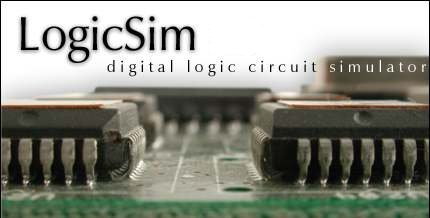
\includegraphics[width=10cm]{../src/logicsim/images/about}
\end{center}

\section{Einleitung}
Der \textit{Logic Simulator}, im folgenden abgekürzt durch \lsN{}, ist der Nachfolger von Andreas Tetzls \lsA{}. \lsA{} ist auf seiner Webseite \url{http://tetzl.de} veröffentlicht.\\

Neue Versionen von \lsN{} sind auf der Webseite \url{http://sis.schule} veröffentlicht. Der Quelltext kann unter GitHub (Projektname: LogicSim3) heruntergeladen werden. Das Programm ist unter der GPL veröffentlicht und darf daher frei verändert werden, sofern der geänderte Quelltext wieder veröffentlicht wird. Eine kommerzielle closed-source Verwendung ist damit ausgeschlossen.\\

Die Entwicklung von \lsA{} wurde seit 11 Jahren nicht mehr fortgeführt, mittlerweile ist die Applet-Technik abgekündigt und ist evtl. bald nicht mehr in den verfügbaren \textit{Java Runtimes} enthalten. Der Autor der fortgeführten Software fehlten einige Funktionen, speziell eine Zoom-Funktion sowie Kopieren und Einfügen von Elementen. Auch konnten keine Beschriftungen zu Ein- und Ausgängen festgelegt werden. Dies war insbesondere bei Modulen problematisch. Auch das Rotieren von Elementen ist noch nicht möglich. Einige dieser Funktionen wurden bereits implementiert. Das Dateiformat wurde auf XML umgestellt, so können die Dateien auch händisch bearbeitet werden.\\

Wichtig für die neue Version war ein Einsatz in der Schule. Da \lsA{} einfach zu bedienen ist und man direkt mit der Modellierung von Schaltkreisen beginnen kann, sollte der Einsatz in der Schule weiter verbessert werden. Die einzelnen >>Gatter<< sind nun in ein Verzeichnis ausgelagert worden und sind damit nicht mehr fest im \textit{Java Archiv} (.jar-Datei) verankert. Dadurch können nun aus didaktischen Gründen einzelne Gatter entfernt werden, um z.B. nur die Grundgatter, Schalter und LEDs zur Verfügung zu stellen.\\

An der Erstellung der Software darf mitgearbeitet werden. Dazu ist das GitHub-Projekt vorhanden. Bitte nehmen Sie daher Kontakt über die GitHub-Projektseite auf.\\

Bitte verwenden Sie auch diesen Weg, falls Sie Fehler der Software melden möchten.\\

\subsection{History}
\begin{tabular}{p{4cm}p{10cm}}
2020-04-03 & Erstellung des Dokuments\\
\end{tabular}

\section{Bedienung}

\subsection{Start}
\lsN{} wird als JAR-Datei ausgeliefert. Hierbei handelt es sich um ein Java-Archiv, dass nur dann lauffähig ist, wenn auf dem Computer JAVA installiert ist. Der Start des Programms geschieht im Normalfall über einen Doppelklick. Sollte dies nicht funktionieren, so kann das Programm auch im Falle von Windows über eine Batchdatei (logicsim.bat) gestartet werden. Sollte auch dies nicht möglich sein, ist evtl. Java nicht korrekt installiert.

\subsection{Grundsätzliche Bedienung}
Die Softwarebedienung erschließt sich in weiten Teilen von selbst. Besonderheiten:
\begin{compactitem}
\item Bauteile werden in die Arbeitsfläche eingefügt, indem es aus der Liste ausgewählt wird. Es wird dann immer in der linken oberen Stelle der Arbeitsfläche positioniert. Bei mehrfachem Anklicken eines Bauteils werden weitere Bauteile versetzt eingefügt.
\item Neue Kabel werden eingefügt, indem stets \textit{ein Ausgang} eines Gatters angeklickt wird. Das freie Kabelende ist immer am Mauszeiger. Jeder weitere Klick auf eine freie Stelle fügt in dem Kabel ein >>Knick<< ein. Ein Kabel wird fertiggestellt, in dem \textit{ein Eingang} eines Bauteils angeklickt wird.\\
Während der Bearbeitung des Kabels kann die Taste \textit{Escape} gedrückt werden, um den zuletzt eingefügten Punkt zu löschen, falls versehentlich ein Punkt platziert wurde.
\item Das Anklicken eines Bauteils oder eines Kabels führt zur Auswahl (\textit{Selektion}) des Teils. Es kann dann per Pfeiltasten oder durch Drag\&Drop mit der Maus verschoben werden. Bei Kabeln werden nur die inneren Punkte bewegt, die äußeren Punkte bleiben an angeschlossenen Bauteile. Werden Bauteilen bewegt, werden entsprechend nur die Kabelenden der angeschlossenen Kabel mitbewegt.
\item Es können mehrere Bauteile ausgewählt werden. Hierzu kann man die Shift-Taste verwenden bei gleichzeitigem Klick auf Bauteile hintereinander, oder der Klick auf die Schaltfläche >>Selekt<< erlaubt das Ziehen eines gestrichelten Kastens um die zu selektierenden Bauteile per Drag\&Drop.
\item Selektierte Bauteile oder Kabel können durch Druck auf die Backspace-Taste (auch Entf- oder Lösch-Taste) entfernt werden. Werden Bauteile gelöscht, so werden automatisch alle angeschlossenen Kabel mitgelöscht.
\item Kabel müssen immer an zwei Enden angeschlossen sein, es gibt keine >>Luftenden<<.
\item Das Mausrad wird unterstützt, Zoomen ist damit möglich, Zusätzlich dazu gibt es passende Schaltflächen zum Vergrößern, Verkleinern und auf den verwendeten Bereich Zoomen.
\end{compactitem}

\subsection{Funktionen - einzeln erläutert}
\lsbild{open}, \lsbild{save}, \lsbild{new}: Dateifunktionen zum öffnen, speichern oder neu erstellen einer Datei.

\lsbild{inputhigh}, \lsbild{inputlow}, \lsbild{inputnorm}, \lsbild{inputinv}: Damit wird ein Eingang eines Gatters modifiziert: als Eingang, der immer HIGH ist, der immer LOW ist, als normaler Eingang oder als invertierter Eingang. DIe Modifikation des Eingangs ist im Schaltplan durch Symbole sichtbar und wirkt sich unmittelbar auf die folgenden Signale aus.

\lsbild{delpoint}, \lsbild{addpoint}: löschen und erstellen einen >>Knickpunkt<< in einem Kabel. Das einmalige Anklicken der Schaltfläche (oder der Auswahl im Menü) erwartet als nächste Aktion ein Klick auf ein Kabel. An der geklickten Stelle wird nun der Knickpunkt gelöscht bzw. ein neuer Punkt eingfügt.

\lsbild{rotate}, \lsbild{mirror}: Rotiert bzw. spiegelt selektierte Bauteile. Es müssen dazu bereits Bauteile ausgewählt sein.

\lsbild{zoomm}, \lsbild{zoomp}: Zoomt herein oder heraus.

\lsbild{select}: Erlaubt das Ziehen eines Kastens um zu selektierende Bauteile. Es werden alle Bauteile ausgewählt, die vollständig im Kasten enthalten sind.

\subsection{Einen Schaltplan erstellen}
Begonnen wird mit der leeren Arbeitsfläche



\subsection{Einsatz in der Schule}
Neu ist das Verzeichnis >>gates<< im Hauptverzeichnis des Programms. In ihm sind kompilierte Klassen, die ihrerseits Gatter und Bauteile für \lsN{} bereitstellen. \lsN{} wird dadurch erweiter- und beschränkbar. Durch Entfernen von Klassendateien aus diesem Verzeichnis sind die entsprechenden Bauteile im Programm nicht mehr verfügbar. So kann in einer Unterrichtsreihe in der Schule zunächst mit Grundkomponenten wie AND, OR, NOT sowie Schaltern und LEDs begonnen werden. Später können dann weitere Komponenten hinzugenommen werden, so dass Schülerinnen und Schülern bei den gewünschten Funktionen bleiben.

\section{Module}
Module sind dort interessant, wo eine Innensicht auf Bauteile gewünscht ist. Es lassen sich z.B. komplexere Bauteile wie Volladdierer oder Schieberegister aus einzelnen Gattern zusammensetzen. Dafür stehen pro Modul immer 16 Ein- und 16 Ausgänge zur Verfügung. Solche Schaltungen lassen sich dann abspeichern und als neue Bauteile als Block verwenden.\\

Neue Module werden über den Menüpunkt >>Neues Modul erstellen<< angelegt. Der Dateiname des Moduls entscheidet dann später über den Eintrag in der Liste der Bauteile links im Programm. Es dürfen zum Test an die Eingänge der \texttt{INPUTS} und an die Ausgänge der \texttt{OUTPUTS} weitere Bauteile angeschlossen werden und auch mit abgespeichert werden. Die Bauteile werden automatisch während der Verwendung als Block automatisch entfernt.
Ein- und Ausgänge von Modulen können Beschriftungen tragen. Diese müssen derzeit noch per Hand eingetragen werden. Wie das geschieht, ist in Abschnitt \ref{labels} beschrieben.

\section{Aufbau der digitalen Schaltungsdateien}
\subsection{Beschriftungen für Ein- und Ausgänge}
\label{labels}

\section{Erweiterung}

\subsection{Verwendung mit Eclipse}
Das Projekt wird derzeit mit Eclipse entwickelt, in der letzten Version. Als Java SDK kommt OpenJDK zum Einsatz.

Da LogicSim zur Entwicklungszeit und zum Start aus Eclipse heraus unbedingt die Verzeichnisse \texttt{circuits} und \texttt{modules} benötigt, ist darauf zu achten, dass diese Ordner zugreifbar sind. Da diese im Eclipse-Projekt-Hauptordner liegen, funktioniert das so.

In der JAR-Datei ist dies anders. Hier gibt es zusätzlich das Verzeichnis \texttt{gates} im Hauptordner, hier müssen die Klassen aus dem \texttt{gates}-Package enthalten sein. Der Vorteil liegt hier in einem einfachen Löschen und Hinzunehmen weiterer Gatter-Typen und Komponenten.

Die Zusammenstellung der Distribution bzw. des LogicSim-ZIP-Archivs erfolgt via ant-build-Skript. Abbildung \ref{projectstructure} zeigt die Dateiansicht aus Eclipse heraus.

\bild{projectstructure}{Struktur des Projekts in der Eclipse-Ansicht}

\subsection{Übersetzung der Texte in andere Sprachen}
Als Muster stehen die Dateien \texttt{de.txt} und \texttt{en.txt} zur Verfügung. Diese Dateien enthalten die neuen Sprachtexte, die von \lsN{} verwendet werden. Vorhandene, andere Sprachdateien sind zwar übersetzt, nur sind die Sprachtextbezeichner noch nicht auf \lsN{} umgestellt.

\subsection{Weiterentwicklung, Implementierung neuer Bauteile}
Eine Erweiterung ist ohne Weiteres möglich. Dazu kann der Source-Tree von Github heruntergeladen werden\footnote{s. im Internet: \url{https://github.com/codepiet/LogicSim3}}. Wird Eclipse verwendet, so kann direkt die Struktur aus Github übernommen werden. Das \textit{src}-Verzeichnis enthält die Quelltexte zum Programm und den Bauteilen. Es sind keine externen Bibliotheken erforderlich.\\

Die Klasse \texttt{App.java} enthält die \texttt{main}-Methode für den Start der Software.
Die Datei \texttt{build.xml} wird für das Generieren von Releases mittels \textit{ant} verwendet.

Da der Aufbau der implementierten Logikgatter sehr einfach ist, können auch Schüler in Facharbeiten weitere, komplexere Gatter implementieren. Die Klasse \texttt{logicsim.Gate} stellt die API, gemeinsam mit der Oberklasse \texttt{logicsim.CircuitPart} bereit. Alle vorhandenen Gatter verwenden lediglich die definierten Methoden. Anhand der vorhandenen Gatterklassen kann das Vorgehen für weiterführende Bauteile abgeschaut werden. Auch Komponenten wie die 7-Segment-Anzeige sind Unterklassen von \texttt{logicsim.Gate}.\\

\section{Nächste Schritte}

\section*{Anhang}
\appendix
\section{Jar-Doppelklick unter Windows 10 einrichten}
Damit der Doppelklick unter einem System funktioniert, müssen die JAR-Dateien einem Programm zugewiesen werden. Oft ist unter Windows 10 der Doppelklick auf Jar-Dateien nicht richtig eingestellt. Ein bloßes Einrichten von >>Öffnen mit<< führt zu keinem Ergebnis. Dies liegt daran, dass dem Programm >>java.exe<<, dass seinerseits die JAR-Datei lädt, ein weiterer Parameter (-jar) mitgegeben werden muss. Dies lässt sich gut über die Registry lösen.

\begin{compactenum}
\item Notieren, wo Java installiert ist, oft in \verb+C:\Programme (x86)\Java\jreXXX\bin\java.exe+
\item >>regedit<< als Administrator ausführen.
\item Zum angegebenen Schlüssel in Abbildung \ref{registryjar1} navigieren.
\item Den Schlüssel wie in Abbildung \ref{registryjar2} angegeben ändern, dabei den richtigen Pfad von Schritt 1 übernehmen.
\end{compactenum}

\bild{registryjar1}{Regedit-Programm mit dargestelltem Pfad zum Schlüssel}
\bild{registryjar2}{Bearbeiten des Schlüssels}

\end{document}